% Options for packages loaded elsewhere
\PassOptionsToPackage{unicode}{hyperref}
\PassOptionsToPackage{hyphens}{url}
\PassOptionsToPackage{dvipsnames,svgnames,x11names}{xcolor}
%
\documentclass[
  11pt,
  letterpaper,
  DIV=11,
  numbers=noendperiod]{scrartcl}

\usepackage{amsmath,amssymb}
\usepackage{iftex}
\ifPDFTeX
  \usepackage[T1]{fontenc}
  \usepackage[utf8]{inputenc}
  \usepackage{textcomp} % provide euro and other symbols
\else % if luatex or xetex
  \usepackage{unicode-math}
  \defaultfontfeatures{Scale=MatchLowercase}
  \defaultfontfeatures[\rmfamily]{Ligatures=TeX,Scale=1}
\fi
\usepackage{lmodern}
\ifPDFTeX\else  
    % xetex/luatex font selection
\fi
% Use upquote if available, for straight quotes in verbatim environments
\IfFileExists{upquote.sty}{\usepackage{upquote}}{}
\IfFileExists{microtype.sty}{% use microtype if available
  \usepackage[]{microtype}
  \UseMicrotypeSet[protrusion]{basicmath} % disable protrusion for tt fonts
}{}
\makeatletter
\@ifundefined{KOMAClassName}{% if non-KOMA class
  \IfFileExists{parskip.sty}{%
    \usepackage{parskip}
  }{% else
    \setlength{\parindent}{0pt}
    \setlength{\parskip}{6pt plus 2pt minus 1pt}}
}{% if KOMA class
  \KOMAoptions{parskip=half}}
\makeatother
\usepackage{xcolor}
\usepackage[a4paper]{geometry}
\setlength{\emergencystretch}{3em} % prevent overfull lines
\setcounter{secnumdepth}{5}
% Make \paragraph and \subparagraph free-standing
\makeatletter
\ifx\paragraph\undefined\else
  \let\oldparagraph\paragraph
  \renewcommand{\paragraph}{
    \@ifstar
      \xxxParagraphStar
      \xxxParagraphNoStar
  }
  \newcommand{\xxxParagraphStar}[1]{\oldparagraph*{#1}\mbox{}}
  \newcommand{\xxxParagraphNoStar}[1]{\oldparagraph{#1}\mbox{}}
\fi
\ifx\subparagraph\undefined\else
  \let\oldsubparagraph\subparagraph
  \renewcommand{\subparagraph}{
    \@ifstar
      \xxxSubParagraphStar
      \xxxSubParagraphNoStar
  }
  \newcommand{\xxxSubParagraphStar}[1]{\oldsubparagraph*{#1}\mbox{}}
  \newcommand{\xxxSubParagraphNoStar}[1]{\oldsubparagraph{#1}\mbox{}}
\fi
\makeatother

\usepackage{color}
\usepackage{fancyvrb}
\newcommand{\VerbBar}{|}
\newcommand{\VERB}{\Verb[commandchars=\\\{\}]}
\DefineVerbatimEnvironment{Highlighting}{Verbatim}{commandchars=\\\{\}}
% Add ',fontsize=\small' for more characters per line
\usepackage{framed}
\definecolor{shadecolor}{RGB}{241,243,245}
\newenvironment{Shaded}{\begin{snugshade}}{\end{snugshade}}
\newcommand{\AlertTok}[1]{\textcolor[rgb]{0.68,0.00,0.00}{#1}}
\newcommand{\AnnotationTok}[1]{\textcolor[rgb]{0.37,0.37,0.37}{#1}}
\newcommand{\AttributeTok}[1]{\textcolor[rgb]{0.40,0.45,0.13}{#1}}
\newcommand{\BaseNTok}[1]{\textcolor[rgb]{0.68,0.00,0.00}{#1}}
\newcommand{\BuiltInTok}[1]{\textcolor[rgb]{0.00,0.23,0.31}{#1}}
\newcommand{\CharTok}[1]{\textcolor[rgb]{0.13,0.47,0.30}{#1}}
\newcommand{\CommentTok}[1]{\textcolor[rgb]{0.37,0.37,0.37}{#1}}
\newcommand{\CommentVarTok}[1]{\textcolor[rgb]{0.37,0.37,0.37}{\textit{#1}}}
\newcommand{\ConstantTok}[1]{\textcolor[rgb]{0.56,0.35,0.01}{#1}}
\newcommand{\ControlFlowTok}[1]{\textcolor[rgb]{0.00,0.23,0.31}{\textbf{#1}}}
\newcommand{\DataTypeTok}[1]{\textcolor[rgb]{0.68,0.00,0.00}{#1}}
\newcommand{\DecValTok}[1]{\textcolor[rgb]{0.68,0.00,0.00}{#1}}
\newcommand{\DocumentationTok}[1]{\textcolor[rgb]{0.37,0.37,0.37}{\textit{#1}}}
\newcommand{\ErrorTok}[1]{\textcolor[rgb]{0.68,0.00,0.00}{#1}}
\newcommand{\ExtensionTok}[1]{\textcolor[rgb]{0.00,0.23,0.31}{#1}}
\newcommand{\FloatTok}[1]{\textcolor[rgb]{0.68,0.00,0.00}{#1}}
\newcommand{\FunctionTok}[1]{\textcolor[rgb]{0.28,0.35,0.67}{#1}}
\newcommand{\ImportTok}[1]{\textcolor[rgb]{0.00,0.46,0.62}{#1}}
\newcommand{\InformationTok}[1]{\textcolor[rgb]{0.37,0.37,0.37}{#1}}
\newcommand{\KeywordTok}[1]{\textcolor[rgb]{0.00,0.23,0.31}{\textbf{#1}}}
\newcommand{\NormalTok}[1]{\textcolor[rgb]{0.00,0.23,0.31}{#1}}
\newcommand{\OperatorTok}[1]{\textcolor[rgb]{0.37,0.37,0.37}{#1}}
\newcommand{\OtherTok}[1]{\textcolor[rgb]{0.00,0.23,0.31}{#1}}
\newcommand{\PreprocessorTok}[1]{\textcolor[rgb]{0.68,0.00,0.00}{#1}}
\newcommand{\RegionMarkerTok}[1]{\textcolor[rgb]{0.00,0.23,0.31}{#1}}
\newcommand{\SpecialCharTok}[1]{\textcolor[rgb]{0.37,0.37,0.37}{#1}}
\newcommand{\SpecialStringTok}[1]{\textcolor[rgb]{0.13,0.47,0.30}{#1}}
\newcommand{\StringTok}[1]{\textcolor[rgb]{0.13,0.47,0.30}{#1}}
\newcommand{\VariableTok}[1]{\textcolor[rgb]{0.07,0.07,0.07}{#1}}
\newcommand{\VerbatimStringTok}[1]{\textcolor[rgb]{0.13,0.47,0.30}{#1}}
\newcommand{\WarningTok}[1]{\textcolor[rgb]{0.37,0.37,0.37}{\textit{#1}}}

\providecommand{\tightlist}{%
  \setlength{\itemsep}{0pt}\setlength{\parskip}{0pt}}\usepackage{longtable,booktabs,array}
\usepackage{calc} % for calculating minipage widths
% Correct order of tables after \paragraph or \subparagraph
\usepackage{etoolbox}
\makeatletter
\patchcmd\longtable{\par}{\if@noskipsec\mbox{}\fi\par}{}{}
\makeatother
% Allow footnotes in longtable head/foot
\IfFileExists{footnotehyper.sty}{\usepackage{footnotehyper}}{\usepackage{footnote}}
\makesavenoteenv{longtable}
\usepackage{graphicx}
\makeatletter
\def\maxwidth{\ifdim\Gin@nat@width>\linewidth\linewidth\else\Gin@nat@width\fi}
\def\maxheight{\ifdim\Gin@nat@height>\textheight\textheight\else\Gin@nat@height\fi}
\makeatother
% Scale images if necessary, so that they will not overflow the page
% margins by default, and it is still possible to overwrite the defaults
% using explicit options in \includegraphics[width, height, ...]{}
\setkeys{Gin}{width=\maxwidth,height=\maxheight,keepaspectratio}
% Set default figure placement to htbp
\makeatletter
\def\fps@figure{htbp}
\makeatother

\usepackage{fvextra} % Enhanced verbatim environment
\DefineVerbatimEnvironment{Highlighting}{Verbatim}{
  breaklines,       % Allow line breaks in long code
  commandchars=\\\{\}, % Command characters for highlighting
  fontsize=\small  % Reduce font size for better fit
}
\KOMAoption{captions}{tableheading}
\makeatletter
\@ifpackageloaded{caption}{}{\usepackage{caption}}
\AtBeginDocument{%
\ifdefined\contentsname
  \renewcommand*\contentsname{Table of contents}
\else
  \newcommand\contentsname{Table of contents}
\fi
\ifdefined\listfigurename
  \renewcommand*\listfigurename{List of Figures}
\else
  \newcommand\listfigurename{List of Figures}
\fi
\ifdefined\listtablename
  \renewcommand*\listtablename{List of Tables}
\else
  \newcommand\listtablename{List of Tables}
\fi
\ifdefined\figurename
  \renewcommand*\figurename{Figure}
\else
  \newcommand\figurename{Figure}
\fi
\ifdefined\tablename
  \renewcommand*\tablename{Table}
\else
  \newcommand\tablename{Table}
\fi
}
\@ifpackageloaded{float}{}{\usepackage{float}}
\floatstyle{ruled}
\@ifundefined{c@chapter}{\newfloat{codelisting}{h}{lop}}{\newfloat{codelisting}{h}{lop}[chapter]}
\floatname{codelisting}{Listing}
\newcommand*\listoflistings{\listof{codelisting}{List of Listings}}
\makeatother
\makeatletter
\makeatother
\makeatletter
\@ifpackageloaded{caption}{}{\usepackage{caption}}
\@ifpackageloaded{subcaption}{}{\usepackage{subcaption}}
\makeatother

\ifLuaTeX
\usepackage[bidi=basic]{babel}
\else
\usepackage[bidi=default]{babel}
\fi
\babelprovide[main,import]{english}
% get rid of language-specific shorthands (see #6817):
\let\LanguageShortHands\languageshorthands
\def\languageshorthands#1{}
\ifLuaTeX
  \usepackage{selnolig}  % disable illegal ligatures
\fi
\usepackage{bookmark}

\IfFileExists{xurl.sty}{\usepackage{xurl}}{} % add URL line breaks if available
\urlstyle{same} % disable monospaced font for URLs
\hypersetup{
  pdftitle={ML\_PS1},
  pdfauthor={Clarice Tee},
  pdflang={en},
  colorlinks=true,
  linkcolor={blue},
  filecolor={Maroon},
  citecolor={Blue},
  urlcolor={Blue},
  pdfcreator={LaTeX via pandoc}}


\title{ML\_PS1}
\author{Clarice Tee}
\date{2025-01-21}

\begin{document}
\maketitle

\RecustomVerbatimEnvironment{verbatim}{Verbatim}{
  showspaces=false,
  showtabs=false,
  breaksymbolleft={},
  breaklines
}

\renewcommand*\contentsname{Table of contents}
{
\hypersetup{linkcolor=}
\setcounter{tocdepth}{3}
\tableofcontents
}

\begin{enumerate}
\def\labelenumi{\arabic{enumi}.}
\tightlist
\item
  Familarize w data
\end{enumerate}

\begin{Shaded}
\begin{Highlighting}[]
\CommentTok{\# Import required libraries}
\ImportTok{import}\NormalTok{ numpy }\ImportTok{as}\NormalTok{ np}
\ImportTok{import}\NormalTok{ os}
\ImportTok{import}\NormalTok{ statsmodels.api }\ImportTok{as}\NormalTok{ sm}
\ImportTok{import}\NormalTok{ pandas }\ImportTok{as}\NormalTok{ pd}
\ImportTok{from}\NormalTok{ sklearn.preprocessing }\ImportTok{import}\NormalTok{ SplineTransformer}
\ImportTok{from}\NormalTok{ sklearn.linear\_model }\ImportTok{import}\NormalTok{ LinearRegression}
\ImportTok{import}\NormalTok{ matplotlib.pyplot }\ImportTok{as}\NormalTok{ plt}
\ImportTok{import}\NormalTok{ seaborn }\ImportTok{as}\NormalTok{ sns}
\ImportTok{from}\NormalTok{ pygam }\ImportTok{import}\NormalTok{ LinearGAM, s, te}
\ImportTok{from}\NormalTok{ sklearn.preprocessing }\ImportTok{import}\NormalTok{ MinMaxScaler}
\ImportTok{from}\NormalTok{ sklearn.model\_selection }\ImportTok{import}\NormalTok{ train\_test\_split}
\ImportTok{from}\NormalTok{ sklearn.metrics }\ImportTok{import}\NormalTok{ mean\_absolute\_error, r2\_score, mean\_squared\_error}
\CommentTok{\# Display all columns in pandas}
\NormalTok{pd.set\_option(}\StringTok{\textquotesingle{}display.max\_columns\textquotesingle{}}\NormalTok{, }\VariableTok{None}\NormalTok{)}
\end{Highlighting}
\end{Shaded}

\begin{Shaded}
\begin{Highlighting}[]
\CommentTok{\# Load the data}
\NormalTok{directory }\OperatorTok{=} \VerbatimStringTok{r"C:\textbackslash{}Users\textbackslash{}clari\textbackslash{}OneDrive\textbackslash{}Documents\textbackslash{}Machine Learning\textbackslash{}mp1"}
\NormalTok{acs\_path }\OperatorTok{=}\NormalTok{ os.path.join(directory, }\StringTok{"acs\_usa.csv"}\NormalTok{)}
\NormalTok{acs\_data }\OperatorTok{=}\NormalTok{ pd.read\_csv(acs\_path)}
\NormalTok{acs\_data.describe()}
\BuiltInTok{print}\NormalTok{(acs\_data.shape)}
\end{Highlighting}
\end{Shaded}

\begin{verbatim}
(9048, 25)
\end{verbatim}

2.a. Make educdc crowsswalk

\begin{Shaded}
\begin{Highlighting}[]
\CommentTok{\# Check unique values of EDUCD in the original data}
\NormalTok{acs\_data[}\StringTok{\textquotesingle{}EDUCD\textquotesingle{}}\NormalTok{].unique()}
\end{Highlighting}
\end{Shaded}

\begin{verbatim}
array([ 65,  71,  63,  64,  81,  50, 114,  40, 101,   2,  61, 115,  26,
        30, 116,  23,  15,  25,  22,  17,  14,  16,  11,  12], dtype=int64)
\end{verbatim}

\begin{Shaded}
\begin{Highlighting}[]
\CommentTok{\# read in crosswalk data}
\NormalTok{crosswalk\_path }\OperatorTok{=}\NormalTok{ os.path.join(directory, }\StringTok{"Education{-}Crosswalk.csv"}\NormalTok{)}
\NormalTok{crosswalk }\OperatorTok{=}\NormalTok{ pd.read\_csv(crosswalk\_path)}
\NormalTok{crosswalk.head()}
\end{Highlighting}
\end{Shaded}

\begin{longtable}[]{@{}lll@{}}
\toprule\noalign{}
& educd & educdc \\
\midrule\noalign{}
\endhead
\bottomrule\noalign{}
\endlastfoot
0 & 2 & 0.0 \\
1 & 10 & 0.0 \\
2 & 11 & 2.0 \\
3 & 12 & 0.0 \\
4 & 13 & 2.5 \\
\end{longtable}

\begin{Shaded}
\begin{Highlighting}[]
\CommentTok{\# Capitalize the column names in the crosswalk }
\NormalTok{crosswalk }\OperatorTok{=}\NormalTok{ crosswalk.rename(columns}\OperatorTok{=}\NormalTok{\{}\StringTok{\textquotesingle{}educd\textquotesingle{}}\NormalTok{: }\StringTok{\textquotesingle{}EDUCD\textquotesingle{}}\NormalTok{, }\StringTok{\textquotesingle{}educdc\textquotesingle{}}\NormalTok{: }\StringTok{\textquotesingle{}EDUCDC\textquotesingle{}}\NormalTok{\})}
\CommentTok{\# map the matching values of EDUCD between the two dataframes (i.e. merge on EDUCD)}

\NormalTok{acs\_data }\OperatorTok{=}\NormalTok{ acs\_data.merge(crosswalk, on}\OperatorTok{=}\StringTok{\textquotesingle{}EDUCD\textquotesingle{}}\NormalTok{, how}\OperatorTok{=}\StringTok{\textquotesingle{}left\textquotesingle{}}\NormalTok{) }

\NormalTok{acs\_data.head()}
\end{Highlighting}
\end{Shaded}

\begin{longtable}[]{@{}lllllllllllllllllllllllllll@{}}
\toprule\noalign{}
& YEAR & SAMPLE & SERIAL & CBSERIAL & HHWT & CLUSTER & STRATA & GQ &
PERNUM & PERWT & NCHILD & SEX & AGE & MARST & RACE & RACED & HISPAN &
HISPAND & EDUC & EDUCD & EMPSTAT & EMPSTATD & INCWAGE & VETSTAT &
VETSTATD & EDUCDC \\
\midrule\noalign{}
\endhead
\bottomrule\noalign{}
\endlastfoot
0 & 2023 & 202301 & 1472 & 2023010069599 & 8100.0 & 2023000014721 &
120201 & 4 & 1 & 8100.0 & 0 & 1 & 19 & 6 & 1 & 100 & 0 & 0 & 6 & 65 & 1
& 12 & 4500 & 1 & 11 & 13.0 \\
1 & 2023 & 202301 & 2120 & 2023010102972 & 648.0 & 2023000021201 &
140401 & 4 & 1 & 648.0 & 0 & 2 & 21 & 6 & 1 & 100 & 0 & 0 & 7 & 71 & 1 &
10 & 5500 & 1 & 11 & 14.0 \\
2 & 2023 & 202301 & 2282 & 2023010110952 & 6642.0 & 2023000022821 &
240001 & 4 & 1 & 6642.0 & 0 & 2 & 18 & 6 & 1 & 100 & 0 & 0 & 6 & 63 & 1
& 14 & 24000 & 1 & 12 & 12.0 \\
3 & 2023 & 202301 & 3578 & 2023010171383 & 43578.0 & 2023000035781 &
80001 & 4 & 1 & 43578.0 & 0 & 1 & 21 & 6 & 1 & 100 & 0 & 0 & 6 & 63 & 1
& 14 & 26000 & 1 & 12 & 12.0 \\
4 & 2023 & 202301 & 3902 & 2023000014636 & 11988.0 & 2023000039021 &
150201 & 1 & 1 & 11826.0 & 2 & 2 & 44 & 4 & 1 & 100 & 0 & 0 & 6 & 65 & 1
& 10 & 40000 & 1 & 11 & 13.0 \\
\end{longtable}

2.b. Making dummy variables

\begin{enumerate}
\def\labelenumi{\roman{enumi}.}
\tightlist
\item
  HIGHSCHOOL 12-15 years of schooling = hs diploma
\end{enumerate}

\begin{Shaded}
\begin{Highlighting}[]
\NormalTok{acs\_data[}\StringTok{\textquotesingle{}HSDIP\textquotesingle{}}\NormalTok{] }\OperatorTok{=}\NormalTok{ np.where((acs\_data[}\StringTok{\textquotesingle{}EDUCDC\textquotesingle{}}\NormalTok{] }\OperatorTok{==} \DecValTok{12}\NormalTok{) }\OperatorTok{|}\NormalTok{ (acs\_data[}\StringTok{\textquotesingle{}EDUCDC\textquotesingle{}}\NormalTok{] }\OperatorTok{==} \DecValTok{13}\NormalTok{) }\OperatorTok{|}\NormalTok{ (acs\_data[}\StringTok{\textquotesingle{}EDUCDC\textquotesingle{}}\NormalTok{] }\OperatorTok{==} \DecValTok{14}\NormalTok{) }\OperatorTok{|}\NormalTok{ (acs\_data[}\StringTok{\textquotesingle{}EDUCDC\textquotesingle{}}\NormalTok{] }\OperatorTok{==} \DecValTok{15}\NormalTok{),}
                             \DecValTok{1}\NormalTok{,}
                             \DecValTok{0}
\NormalTok{                             )}
\end{Highlighting}
\end{Shaded}

\begin{enumerate}
\def\labelenumi{\roman{enumi}.}
\setcounter{enumi}{1}
\tightlist
\item
  COLLEGE \#if more than 16 years of schooling, has college diploma daw
\end{enumerate}

\begin{Shaded}
\begin{Highlighting}[]
\NormalTok{acs\_data[}\StringTok{\textquotesingle{}COLDIP\textquotesingle{}}\NormalTok{] }\OperatorTok{=}\NormalTok{ np.where((acs\_data[}\StringTok{\textquotesingle{}EDUCDC\textquotesingle{}}\NormalTok{] }\OperatorTok{\textgreater{}=} \DecValTok{16}\NormalTok{),}
    \DecValTok{1}\NormalTok{,}
    \DecValTok{0}
\NormalTok{)}
\end{Highlighting}
\end{Shaded}

\begin{enumerate}
\def\labelenumi{\roman{enumi}.}
\setcounter{enumi}{2}
\tightlist
\item
  \& iv. RACE
\end{enumerate}

\begin{Shaded}
\begin{Highlighting}[]
\CommentTok{\# WHITE = 1, 0 othewise. BLACK =1, 0 otherwise}
\NormalTok{acs\_data[}\StringTok{\textquotesingle{}WHITE\textquotesingle{}}\NormalTok{] }\OperatorTok{=}\NormalTok{ np.where(acs\_data[}\StringTok{\textquotesingle{}RACE\textquotesingle{}}\NormalTok{] }\OperatorTok{==} \DecValTok{1}\NormalTok{, }\DecValTok{1}\NormalTok{, }\DecValTok{0}\NormalTok{)}
\NormalTok{acs\_data[}\StringTok{\textquotesingle{}BLACK\textquotesingle{}}\NormalTok{] }\OperatorTok{=}\NormalTok{ np.where(acs\_data[}\StringTok{\textquotesingle{}RACE\textquotesingle{}}\NormalTok{] }\OperatorTok{==} \DecValTok{2}\NormalTok{, }\DecValTok{1}\NormalTok{, }\DecValTok{0}\NormalTok{)}
\end{Highlighting}
\end{Shaded}

\begin{enumerate}
\def\labelenumi{\alph{enumi}.}
\setcounter{enumi}{21}
\tightlist
\item
  HISPANIC
\end{enumerate}

\begin{Shaded}
\begin{Highlighting}[]
\NormalTok{acs\_data[}\StringTok{\textquotesingle{}HISPANIC\textquotesingle{}}\NormalTok{] }\OperatorTok{=}\NormalTok{ np.where((acs\_data[}\StringTok{\textquotesingle{}HISPAN\textquotesingle{}}\NormalTok{] }\OperatorTok{==} \DecValTok{1}\NormalTok{) }\OperatorTok{|}\NormalTok{ (acs\_data[}\StringTok{\textquotesingle{}HISPAN\textquotesingle{}}\NormalTok{] }\OperatorTok{==} \DecValTok{2}\NormalTok{) }\OperatorTok{|}\NormalTok{ (acs\_data[}\StringTok{\textquotesingle{}HISPAN\textquotesingle{}}\NormalTok{] }\OperatorTok{==} \DecValTok{3}\NormalTok{) }\OperatorTok{|}\NormalTok{ (acs\_data[}\StringTok{\textquotesingle{}HISPAN\textquotesingle{}}\NormalTok{] }\OperatorTok{==} \DecValTok{4}\NormalTok{),}
    \DecValTok{1}\NormalTok{,}
    \DecValTok{0}
\NormalTok{)}
\end{Highlighting}
\end{Shaded}

\begin{enumerate}
\def\labelenumi{\roman{enumi}.}
\setcounter{enumi}{5}
\tightlist
\item
  MARRIED
\end{enumerate}

\begin{Shaded}
\begin{Highlighting}[]
\NormalTok{acs\_data[}\StringTok{\textquotesingle{}MAR\textquotesingle{}}\NormalTok{] }\OperatorTok{=}\NormalTok{ np.where(}
\NormalTok{    (acs\_data[}\StringTok{\textquotesingle{}MARST\textquotesingle{}}\NormalTok{] }\OperatorTok{==} \DecValTok{1}\NormalTok{) }\OperatorTok{|}\NormalTok{ (acs\_data[}\StringTok{\textquotesingle{}MARST\textquotesingle{}}\NormalTok{] }\OperatorTok{==} \DecValTok{2}\NormalTok{),}
    \DecValTok{1}\NormalTok{,}
    \DecValTok{0}
\NormalTok{)}
\end{Highlighting}
\end{Shaded}

\begin{enumerate}
\def\labelenumi{\roman{enumi}.}
\setcounter{enumi}{6}
\tightlist
\item
  FEMALE
\end{enumerate}

\begin{Shaded}
\begin{Highlighting}[]
\NormalTok{acs\_data[}\StringTok{\textquotesingle{}SEX\textquotesingle{}}\NormalTok{].unique()}
\NormalTok{acs\_data[}\StringTok{\textquotesingle{}FEMALE\textquotesingle{}}\NormalTok{] }\OperatorTok{=}\NormalTok{ np.where(acs\_data[}\StringTok{\textquotesingle{}SEX\textquotesingle{}}\NormalTok{] }\OperatorTok{==} \DecValTok{2}\NormalTok{, }\DecValTok{1}\NormalTok{, }\DecValTok{0}\NormalTok{)}
\end{Highlighting}
\end{Shaded}

\begin{enumerate}
\def\labelenumi{\roman{enumi}.}
\setcounter{enumi}{7}
\tightlist
\item
  VET (1 = VET, 0 = NOT)
\end{enumerate}

\begin{Shaded}
\begin{Highlighting}[]
\NormalTok{acs\_data[}\StringTok{\textquotesingle{}VET\textquotesingle{}}\NormalTok{] }\OperatorTok{=}\NormalTok{ np.where(acs\_data[}\StringTok{\textquotesingle{}VETSTAT\textquotesingle{}}\NormalTok{] }\OperatorTok{==} \DecValTok{2}\NormalTok{, }\DecValTok{1}\NormalTok{, }\DecValTok{0}\NormalTok{)}
\end{Highlighting}
\end{Shaded}

2.c.Interaction term Create an interaction between each of the education
dummy variables (hsdip and coldip) and the continuous measure of
education (educdc

\begin{Shaded}
\begin{Highlighting}[]
\NormalTok{acs\_data[}\StringTok{\textquotesingle{}HSDIP\_EDUCDC\textquotesingle{}}\NormalTok{] }\OperatorTok{=}\NormalTok{ acs\_data[}\StringTok{\textquotesingle{}HSDIP\textquotesingle{}}\NormalTok{] }\OperatorTok{*}\NormalTok{ acs\_data[}\StringTok{\textquotesingle{}EDUCDC\textquotesingle{}}\NormalTok{]}
\NormalTok{acs\_data[}\StringTok{\textquotesingle{}COLDIP\_EDUCDC\textquotesingle{}}\NormalTok{] }\OperatorTok{=}\NormalTok{ acs\_data[}\StringTok{\textquotesingle{}COLDIP\textquotesingle{}}\NormalTok{] }\OperatorTok{*}\NormalTok{ acs\_data[}\StringTok{\textquotesingle{}EDUCDC\textquotesingle{}}\NormalTok{]}
\end{Highlighting}
\end{Shaded}

2.d. Create vairables

Age squared

\begin{Shaded}
\begin{Highlighting}[]
\CommentTok{\# creating new variable "AGEQ" in the data, which is the square of AGE}
\NormalTok{acs\_data[}\StringTok{\textquotesingle{}AGEQ\textquotesingle{}}\NormalTok{] }\OperatorTok{=}\NormalTok{ np.power(acs\_data[}\StringTok{\textquotesingle{}AGE\textquotesingle{}}\NormalTok{], }\DecValTok{2}\NormalTok{)}
\end{Highlighting}
\end{Shaded}

The natural log of incwage

\begin{Shaded}
\begin{Highlighting}[]
\CommentTok{\# We first drop those with 0 income. This is because ln(0) is undefined}
\NormalTok{acs\_data }\OperatorTok{=}\NormalTok{ acs\_data[acs\_data.INCWAGE }\OperatorTok{!=} \DecValTok{0}\NormalTok{]}
\CommentTok{\# creating new variable "INCWAGE\_log" in the data, the natural log of INCWAGE }
\NormalTok{acs\_data[}\StringTok{\textquotesingle{}LNINCWAGE\textquotesingle{}}\NormalTok{] }\OperatorTok{=}\NormalTok{ np.log(acs\_data[}\StringTok{\textquotesingle{}INCWAGE\textquotesingle{}}\NormalTok{])}
\end{Highlighting}
\end{Shaded}

\begin{Shaded}
\begin{Highlighting}[]
\NormalTok{acs\_data[[}\StringTok{\textquotesingle{}INCWAGE\textquotesingle{}}\NormalTok{,}\StringTok{\textquotesingle{}LNINCWAGE\textquotesingle{}}\NormalTok{]].head(}\DecValTok{10}\NormalTok{)}
\end{Highlighting}
\end{Shaded}

\begin{longtable}[]{@{}lll@{}}
\toprule\noalign{}
& INCWAGE & LNINCWAGE \\
\midrule\noalign{}
\endhead
\bottomrule\noalign{}
\endlastfoot
0 & 4500 & 8.411833 \\
1 & 5500 & 8.612503 \\
2 & 24000 & 10.085809 \\
3 & 26000 & 10.165852 \\
4 & 40000 & 10.596635 \\
5 & 70000 & 11.156251 \\
6 & 60000 & 11.002100 \\
7 & 30000 & 10.308953 \\
8 & 5000 & 8.517193 \\
9 & 118000 & 11.678440 \\
\end{longtable}

\subsection{Data Analysis Questions}\label{data-analysis-questions}

4.1 Compute descriptive (summary) statistics for the following
variables: year, incwage, lnincwage, educdc, f emale, age, ageq, white,
black, hispanic, married, nchild, vet, hsdip, coldip, and the
interaction terms. In other words, compute sample means, standard
deviations, etc.

\begin{Shaded}
\begin{Highlighting}[]
\KeywordTok{def}\NormalTok{ acs\_summary\_statistics(data, variables):}

\NormalTok{    acs\_summary\_stats }\OperatorTok{=}\NormalTok{ []}

    \ControlFlowTok{for}\NormalTok{ var }\KeywordTok{in}\NormalTok{ variables:}
        \ControlFlowTok{if}\NormalTok{ var }\KeywordTok{in}\NormalTok{ data.columns:  }\CommentTok{\# Ensure the variable exists in the DataFrame}
\NormalTok{            stats }\OperatorTok{=}\NormalTok{ \{}
                \StringTok{\textquotesingle{}Variable\textquotesingle{}}\NormalTok{: var,}
                \StringTok{\textquotesingle{}Mean\textquotesingle{}}\NormalTok{: data[var].mean(),}
                \StringTok{\textquotesingle{}Std Dev\textquotesingle{}}\NormalTok{: data[var].std(),}
                \StringTok{\textquotesingle{}Min\textquotesingle{}}\NormalTok{: data[var].}\BuiltInTok{min}\NormalTok{(),}
                \StringTok{\textquotesingle{}Max\textquotesingle{}}\NormalTok{: data[var].}\BuiltInTok{max}\NormalTok{(),}
                \StringTok{\textquotesingle{}Count\textquotesingle{}}\NormalTok{: data[var].count()}
\NormalTok{            \}}
\NormalTok{            acs\_summary\_stats.append(stats)}

    \CommentTok{\# Convert summary stats to a DataFrame}
    \ControlFlowTok{return}\NormalTok{ pd.DataFrame(acs\_summary\_stats)}


\CommentTok{\# List of variables to compute summary statistics for}
\NormalTok{variables }\OperatorTok{=}\NormalTok{ [}
    \StringTok{\textquotesingle{}YEAR\textquotesingle{}}\NormalTok{, }\StringTok{\textquotesingle{}INCWAGE\textquotesingle{}}\NormalTok{, }\StringTok{\textquotesingle{}LNINCWAGE\textquotesingle{}}\NormalTok{, }\StringTok{\textquotesingle{}EDUCDC\textquotesingle{}}\NormalTok{, }\StringTok{\textquotesingle{}FEMALE\textquotesingle{}}\NormalTok{, }\StringTok{\textquotesingle{}AGE\textquotesingle{}}\NormalTok{, }\StringTok{\textquotesingle{}AGEQ\textquotesingle{}}\NormalTok{,}
    \StringTok{\textquotesingle{}WHITE\textquotesingle{}}\NormalTok{, }\StringTok{\textquotesingle{}BLACK\textquotesingle{}}\NormalTok{, }\StringTok{\textquotesingle{}HISPANIC\textquotesingle{}}\NormalTok{, }\StringTok{\textquotesingle{}MAR\textquotesingle{}}\NormalTok{, }\StringTok{\textquotesingle{}NCHILD\textquotesingle{}}\NormalTok{, }\StringTok{\textquotesingle{}VET\textquotesingle{}}\NormalTok{,}
    \StringTok{\textquotesingle{}HSDIP\textquotesingle{}}\NormalTok{, }\StringTok{\textquotesingle{}COLDIP\textquotesingle{}}\NormalTok{, }\StringTok{\textquotesingle{}HSDIP\_EDUCDC\textquotesingle{}}\NormalTok{, }\StringTok{\textquotesingle{}COLDIP\_EDUCDC\textquotesingle{}}
\NormalTok{]}

\CommentTok{\# Call function}
\NormalTok{acs\_summary\_stats }\OperatorTok{=}\NormalTok{ acs\_summary\_statistics(acs\_data, variables)}

\CommentTok{\# Display the results with formatting}
\NormalTok{pd.set\_option(}\StringTok{\textquotesingle{}display.float\_format\textquotesingle{}}\NormalTok{, }\KeywordTok{lambda}\NormalTok{ x: }\StringTok{\textquotesingle{}}\SpecialCharTok{\%.3f}\StringTok{\textquotesingle{}} \OperatorTok{\%}\NormalTok{ x) }
\BuiltInTok{print}\NormalTok{(acs\_summary\_stats.to\_string(index}\OperatorTok{=}\VariableTok{False}\NormalTok{))  }
\end{Highlighting}
\end{Shaded}

\begin{verbatim}
     Variable      Mean   Std Dev      Min        Max  Count
         YEAR  2023.000     0.000 2023.000   2023.000   8610
      INCWAGE 70235.557 82434.439   20.000 770000.000   8610
    LNINCWAGE    10.693     1.079    2.996     13.554   8610
       EDUCDC    14.310     3.054    0.000     22.000   8610
       FEMALE     0.488     0.500    0.000      1.000   8610
          AGE    41.627    13.291   18.000     65.000   8610
         AGEQ  1909.434  1118.953  324.000   4225.000   8610
        WHITE     0.663     0.473    0.000      1.000   8610
        BLACK     0.082     0.275    0.000      1.000   8610
     HISPANIC     0.163     0.370    0.000      1.000   8610
          MAR     0.557     0.497    0.000      1.000   8610
       NCHILD     0.780     1.097    0.000      6.000   8610
          VET     0.041     0.198    0.000      1.000   8610
        HSDIP     0.537     0.499    0.000      1.000   8610
       COLDIP     0.415     0.493    0.000      1.000   8610
 HSDIP_EDUCDC     6.939     6.484    0.000     14.000   8610
COLDIP_EDUCDC     7.060     8.435    0.000     22.000   8610
\end{verbatim}

4.2 Scatter plot ln (incwage) and EDUCDC. Include a linear fit line. Be
sure to label all axes and include an informative title.

\begin{Shaded}
\begin{Highlighting}[]
\CommentTok{\# Extract data for the scatter plot}
\NormalTok{X }\OperatorTok{=}\NormalTok{ acs\_data[[}\StringTok{\textquotesingle{}EDUCDC\textquotesingle{}}\NormalTok{]].values}
\NormalTok{y }\OperatorTok{=}\NormalTok{ acs\_data[}\StringTok{\textquotesingle{}LNINCWAGE\textquotesingle{}}\NormalTok{].values}
\CommentTok{\# Fit a linear regression model}
\NormalTok{model }\OperatorTok{=}\NormalTok{ LinearRegression()}
\NormalTok{model.fit(X, y)}
\NormalTok{y\_pred }\OperatorTok{=}\NormalTok{ model.predict(X) }

\CommentTok{\# Create a figure and axis object}
\NormalTok{fig, ax }\OperatorTok{=}\NormalTok{ plt.subplots(figsize}\OperatorTok{=}\NormalTok{(}\DecValTok{10}\NormalTok{, }\DecValTok{6}\NormalTok{))}

\CommentTok{\# Scatterplot of education vs. log income}
\NormalTok{ax.scatter(acs\_data[}\StringTok{\textquotesingle{}EDUCDC\textquotesingle{}}\NormalTok{], acs\_data[}\StringTok{\textquotesingle{}LNINCWAGE\textquotesingle{}}\NormalTok{],}
\NormalTok{           alpha}\OperatorTok{=}\FloatTok{0.6}\NormalTok{, s}\OperatorTok{=}\DecValTok{30}\NormalTok{, label}\OperatorTok{=}\StringTok{\textquotesingle{}Data Points\textquotesingle{}}\NormalTok{)}

\CommentTok{\# Linear fit line}
\NormalTok{ax.plot(acs\_data[}\StringTok{\textquotesingle{}EDUCDC\textquotesingle{}}\NormalTok{], y\_pred, color}\OperatorTok{=}\StringTok{"red"}\NormalTok{,}
\NormalTok{        linewidth}\OperatorTok{=}\DecValTok{2}\NormalTok{, label}\OperatorTok{=}\StringTok{"Linear Fit"}\NormalTok{)}

\CommentTok{\# Setting the title, legend, and labels}
\NormalTok{ax.set\_title(}
    \StringTok{\textquotesingle{}Scatter Plot of Log Income (LNINCWAGE) and Education (EDUCDC)\textquotesingle{}}\NormalTok{, fontsize}\OperatorTok{=}\DecValTok{14}\NormalTok{)}
\NormalTok{ax.set\_xlabel(}\StringTok{\textquotesingle{}Years of Education (EDUCDC)\textquotesingle{}}\NormalTok{, fontsize}\OperatorTok{=}\DecValTok{12}\NormalTok{)}
\NormalTok{ax.set\_ylabel(}\StringTok{\textquotesingle{}Log Income (LNINCWAGE)\textquotesingle{}}\NormalTok{, fontsize}\OperatorTok{=}\DecValTok{12}\NormalTok{)}
\NormalTok{ax.legend()}
\NormalTok{ax.grid(alpha}\OperatorTok{=}\FloatTok{0.3}\NormalTok{)}


\NormalTok{plt.show()}
\end{Highlighting}
\end{Shaded}

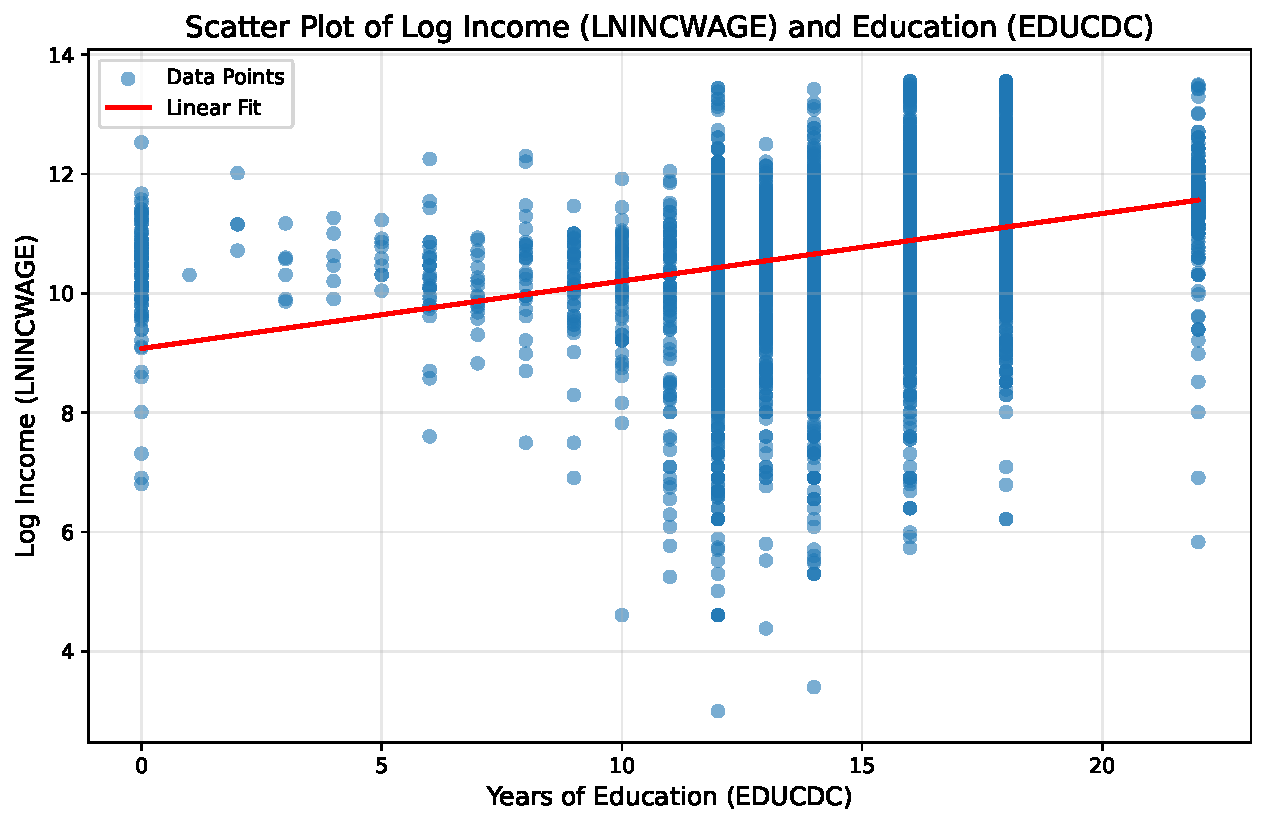
\includegraphics{mp1_files/figure-pdf/cell-19-output-1.pdf}

4.3 LNINCWAGE MODEL

\begin{Shaded}
\begin{Highlighting}[]
\ImportTok{import}\NormalTok{ statsmodels.formula.api }\ImportTok{as}\NormalTok{ smf}

\NormalTok{LNINCWAGE\_reg }\OperatorTok{=}\NormalTok{ smf.ols(}
    \StringTok{\textquotesingle{}LNINCWAGE \textasciitilde{} EDUCDC + FEMALE + AGE + AGEQ + WHITE + BLACK + HISPANIC+ MAR + NCHILD + VET\textquotesingle{}}\NormalTok{, data}\OperatorTok{=}\NormalTok{acs\_data).fit()}
\BuiltInTok{print}\NormalTok{(LNINCWAGE\_reg.summary())}
\end{Highlighting}
\end{Shaded}

\begin{verbatim}
                            OLS Regression Results                            
==============================================================================
Dep. Variable:              LNINCWAGE   R-squared:                       0.282
Model:                            OLS   Adj. R-squared:                  0.281
Method:                 Least Squares   F-statistic:                     337.3
Date:                Thu, 30 Jan 2025   Prob (F-statistic):               0.00
Time:                        22:58:05   Log-Likelihood:                -11445.
No. Observations:                8610   AIC:                         2.291e+04
Df Residuals:                    8599   BIC:                         2.299e+04
Df Model:                          10                                         
Covariance Type:            nonrobust                                         
==============================================================================
                 coef    std err          t      P>|t|      [0.025      0.975]
------------------------------------------------------------------------------
Intercept      6.1306      0.116     52.856      0.000       5.903       6.358
EDUCDC         0.0994      0.003     29.325      0.000       0.093       0.106
FEMALE        -0.3832      0.020    -19.100      0.000      -0.423      -0.344
AGE            0.1493      0.006     26.016      0.000       0.138       0.161
AGEQ          -0.0016   6.76e-05    -23.066      0.000      -0.002      -0.001
WHITE         -0.0070      0.028     -0.253      0.801      -0.061       0.047
BLACK         -0.1202      0.043     -2.791      0.005      -0.205      -0.036
HISPANIC      -0.0211      0.033     -0.640      0.522      -0.086       0.043
MAR            0.2053      0.023      8.867      0.000       0.160       0.251
NCHILD        -0.0082      0.010     -0.794      0.427      -0.028       0.012
VET           -0.0132      0.050     -0.261      0.794      -0.112       0.086
==============================================================================
Omnibus:                     2566.758   Durbin-Watson:                   1.845
Prob(Omnibus):                  0.000   Jarque-Bera (JB):            11879.119
Skew:                          -1.379   Prob(JB):                         0.00
Kurtosis:                       8.050   Cond. No.                     2.62e+04
==============================================================================

Notes:
[1] Standard Errors assume that the covariance matrix of the errors is correctly specified.
[2] The condition number is large, 2.62e+04. This might indicate that there are
strong multicollinearity or other numerical problems.
\end{verbatim}

4.3.a The model explains 28.1\% of the variation in log wages (adjusted
r2 value)

4.3.b. (b) What is the return to an additional year of education?11 Is
this statistically significant?Is it practically significant? Briefly
explain. note that your answer should be in terms of wages, not log
wages.

\begin{Shaded}
\begin{Highlighting}[]
\NormalTok{beta\_EDUCDC }\OperatorTok{=}\NormalTok{ LNINCWAGE\_reg.params.iloc[}\DecValTok{1}\NormalTok{]}

\CommentTok{\# Convert}
\NormalTok{change\_wages\_EDUCDC }\OperatorTok{=}\NormalTok{ (np.exp(beta\_EDUCDC) }\OperatorTok{{-}} \DecValTok{1}\NormalTok{) }\OperatorTok{*} \DecValTok{100}

\NormalTok{mean\_wage }\OperatorTok{=}\NormalTok{ acs\_data[}\StringTok{\textquotesingle{}INCWAGE\textquotesingle{}}\NormalTok{].mean()  }\CommentTok{\# Calculate mean directly from the data}

\CommentTok{\# Calculate dollar change}
\NormalTok{dollar\_change\_EDUCDC }\OperatorTok{=}\NormalTok{ mean\_wage }\OperatorTok{*}\NormalTok{ (change\_wages\_EDUCDC }\OperatorTok{/} \DecValTok{100}\NormalTok{)}

\BuiltInTok{print}\NormalTok{(}\StringTok{"Additional year of education means a 10.45 percent increase in wages. Dollar change in wages for an additional year of education is:"}\NormalTok{, dollar\_change\_EDUCDC)}
\end{Highlighting}
\end{Shaded}

\begin{verbatim}
Additional year of education means a 10.45 percent increase in wages. Dollar change in wages for an additional year of education is: 7341.363608190367
\end{verbatim}

Based on the p-value, it is statistically significant at the 1\% level.

4.3.c.

Here, we need to take the derivative of the model w rt AGE and equate it
to 0. We are left with Beta(3) + 2Beta(4)AGE

\begin{Shaded}
\begin{Highlighting}[]
\CommentTok{\# Getting the coefficients for AGE and AGE\^{}2}
\NormalTok{beta\_AGE }\OperatorTok{=}\NormalTok{ LNINCWAGE\_reg.params.iloc[}\DecValTok{3}\NormalTok{]      }
\NormalTok{beta\_AGE2 }\OperatorTok{=}\NormalTok{ LNINCWAGE\_reg.params.iloc[}\DecValTok{4}\NormalTok{]  }

\CommentTok{\# Calculate the age at which the highest wage occurs}
\NormalTok{max\_age }\OperatorTok{=} \OperatorTok{{-}}\NormalTok{beta\_AGE }\OperatorTok{/}\NormalTok{ (}\DecValTok{2} \OperatorTok{*}\NormalTok{ beta\_AGE2)}
\BuiltInTok{print}\NormalTok{(max\_age)}
\end{Highlighting}
\end{Shaded}

\begin{verbatim}
47.861998868799084
\end{verbatim}

We must check whether this is a local max or minumum by taking the
second derivative wrt age, leaving us w 2Beta(4).

\begin{Shaded}
\begin{Highlighting}[]
\NormalTok{second\_deriv }\OperatorTok{=}\NormalTok{ (}\DecValTok{2} \OperatorTok{*}\NormalTok{ beta\_AGE2)}
\BuiltInTok{print}\NormalTok{(second\_deriv)}
\end{Highlighting}
\end{Shaded}

\begin{verbatim}
-0.0031195396677629757
\end{verbatim}

Now that we know it is negative, we know this is the maximum. therefore:

\begin{Shaded}
\begin{Highlighting}[]
\BuiltInTok{print}\NormalTok{(}\SpecialStringTok{f"The age at which the model predicts the highest wage is approximately 48 years."}\NormalTok{)}
\end{Highlighting}
\end{Shaded}

\begin{verbatim}
The age at which the model predicts the highest wage is approximately 48 years.
\end{verbatim}

4.3.d.

\begin{Shaded}
\begin{Highlighting}[]
\CommentTok{\# Getting the Coefficient for FEMALE}
\NormalTok{beta\_female }\OperatorTok{=}\NormalTok{ LNINCWAGE\_reg.params.iloc[}\DecValTok{2}\NormalTok{]   }

\CommentTok{\# Convert log{-}wage to percentage change}
\NormalTok{percentage\_change\_female }\OperatorTok{=}\NormalTok{ (np.exp(beta\_female) }\OperatorTok{{-}} \DecValTok{1}\NormalTok{) }\OperatorTok{*} \DecValTok{100}

\BuiltInTok{print}\NormalTok{(}\SpecialStringTok{f"Being female is associated with a }\SpecialCharTok{\{}\NormalTok{percentage\_change\_female}\SpecialCharTok{:.1f\}}\SpecialStringTok{\% change in wages."}\NormalTok{)}
\end{Highlighting}
\end{Shaded}

\begin{verbatim}
Being female is associated with a -31.8% change in wages.
\end{verbatim}

The model predicts that being a women means that, all else equal, wages
are lower by about 31.8\%. This makes sense because of gender
discrimination against women, where their work is undervalued relative
to men or they may take lower paying jobs due to having to work
part-time to take on child rearing work.

4.3.e. All else equal, white individuals have approximately a .7\%
decrease in their wages compared to other races, although, this is not
significant because we cannot even reject the null hypothesis at a
significance level of 10\%.

All else equal, black individuals have 12.02\% less than other races and
this proves to be a significant value at the 1\% level.

4.4

\begin{Shaded}
\begin{Highlighting}[]
\CommentTok{\#\# Create degree groups}
\NormalTok{acs\_data[}\StringTok{\textquotesingle{}GROUP\textquotesingle{}}\NormalTok{] }\OperatorTok{=} \StringTok{\textquotesingle{}No High School Diploma\textquotesingle{}}  \CommentTok{\# Default group}
\NormalTok{acs\_data.loc[(acs\_data[}\StringTok{\textquotesingle{}HSDIP\textquotesingle{}}\NormalTok{] }\OperatorTok{==} \DecValTok{1}\NormalTok{) }\OperatorTok{\&}\NormalTok{ (acs\_data[}\StringTok{\textquotesingle{}COLDIP\textquotesingle{}}\NormalTok{] }\OperatorTok{==} \DecValTok{0}\NormalTok{), }\StringTok{\textquotesingle{}GROUP\textquotesingle{}}\NormalTok{] }\OperatorTok{=} \StringTok{\textquotesingle{}High School Diploma\textquotesingle{}}
\NormalTok{acs\_data.loc[(acs\_data[}\StringTok{\textquotesingle{}COLDIP\textquotesingle{}}\NormalTok{] }\OperatorTok{==} \DecValTok{1}\NormalTok{), }\StringTok{\textquotesingle{}GROUP\textquotesingle{}}\NormalTok{] }\OperatorTok{=} \StringTok{\textquotesingle{}College Degree\textquotesingle{}}

\CommentTok{\# Create the plot}
\NormalTok{plt.figure(figsize}\OperatorTok{=}\NormalTok{(}\DecValTok{12}\NormalTok{, }\DecValTok{8}\NormalTok{))}

\CommentTok{\# Colors per grp}
\NormalTok{group\_colors }\OperatorTok{=}\NormalTok{ \{}
    \StringTok{\textquotesingle{}No High School Diploma\textquotesingle{}}\NormalTok{: }\StringTok{\textquotesingle{}orange\textquotesingle{}}\NormalTok{,}
    \StringTok{\textquotesingle{}High School Diploma\textquotesingle{}}\NormalTok{: }\StringTok{\textquotesingle{}green\textquotesingle{}}\NormalTok{,}
    \StringTok{\textquotesingle{}College Degree\textquotesingle{}}\NormalTok{: }\StringTok{\textquotesingle{}blue\textquotesingle{}}
\NormalTok{\}}

\CommentTok{\# Plot scatter points and regression lines for each group}
\ControlFlowTok{for}\NormalTok{ group, color }\KeywordTok{in}\NormalTok{ group\_colors.items():}
\NormalTok{    subset }\OperatorTok{=}\NormalTok{ acs\_data[acs\_data[}\StringTok{\textquotesingle{}GROUP\textquotesingle{}}\NormalTok{] }\OperatorTok{==}\NormalTok{ group]  }\CommentTok{\# Filter data for each group}
    
    \CommentTok{\# Scatterplot for this group}
\NormalTok{    sns.scatterplot(}
\NormalTok{        x}\OperatorTok{=}\StringTok{\textquotesingle{}EDUCDC\textquotesingle{}}\NormalTok{, }
\NormalTok{        y}\OperatorTok{=}\StringTok{\textquotesingle{}LNINCWAGE\textquotesingle{}}\NormalTok{,}
\NormalTok{        data}\OperatorTok{=}\NormalTok{subset, }
\NormalTok{        color}\OperatorTok{=}\NormalTok{color, }
\NormalTok{        alpha}\OperatorTok{=}\FloatTok{0.6}\NormalTok{, }
\NormalTok{        label}\OperatorTok{=}\NormalTok{group}
\NormalTok{    )}
    
    \CommentTok{\# Regression line for this group}
\NormalTok{    sns.regplot(}
\NormalTok{        x}\OperatorTok{=}\StringTok{\textquotesingle{}EDUCDC\textquotesingle{}}\NormalTok{, }
\NormalTok{        y}\OperatorTok{=}\StringTok{\textquotesingle{}LNINCWAGE\textquotesingle{}}\NormalTok{,  }
\NormalTok{        data}\OperatorTok{=}\NormalTok{subset, }
\NormalTok{        scatter}\OperatorTok{=}\VariableTok{False}\NormalTok{, }
\NormalTok{        color}\OperatorTok{=}\NormalTok{color, }
\NormalTok{        line\_kws}\OperatorTok{=}\NormalTok{\{}\StringTok{\textquotesingle{}linewidth\textquotesingle{}}\NormalTok{: }\DecValTok{2}\NormalTok{\},}
\NormalTok{        truncate}\OperatorTok{=}\VariableTok{True}
\NormalTok{    )}

\CommentTok{\# Add labels, title, and legend}
\NormalTok{plt.title(}\StringTok{\textquotesingle{}Log Income Wage) vs. Education (EDUCDC)\textquotesingle{}}\NormalTok{, fontsize}\OperatorTok{=}\DecValTok{16}\NormalTok{)}
\NormalTok{plt.xlabel(}\StringTok{\textquotesingle{}Years of Education (EDUCDC)\textquotesingle{}}\NormalTok{, fontsize}\OperatorTok{=}\DecValTok{14}\NormalTok{)}
\NormalTok{plt.ylabel(}\StringTok{\textquotesingle{}Log Income (LNINCWAGE)\textquotesingle{}}\NormalTok{, fontsize}\OperatorTok{=}\DecValTok{14}\NormalTok{)  }\CommentTok{\# Fix label}
\NormalTok{plt.legend(title}\OperatorTok{=}\StringTok{\textquotesingle{}GROUP\textquotesingle{}}\NormalTok{, fontsize}\OperatorTok{=}\DecValTok{12}\NormalTok{)}
\NormalTok{plt.grid(alpha}\OperatorTok{=}\FloatTok{0.3}\NormalTok{)}

\CommentTok{\# Show the plot}
\NormalTok{plt.show()}
\end{Highlighting}
\end{Shaded}

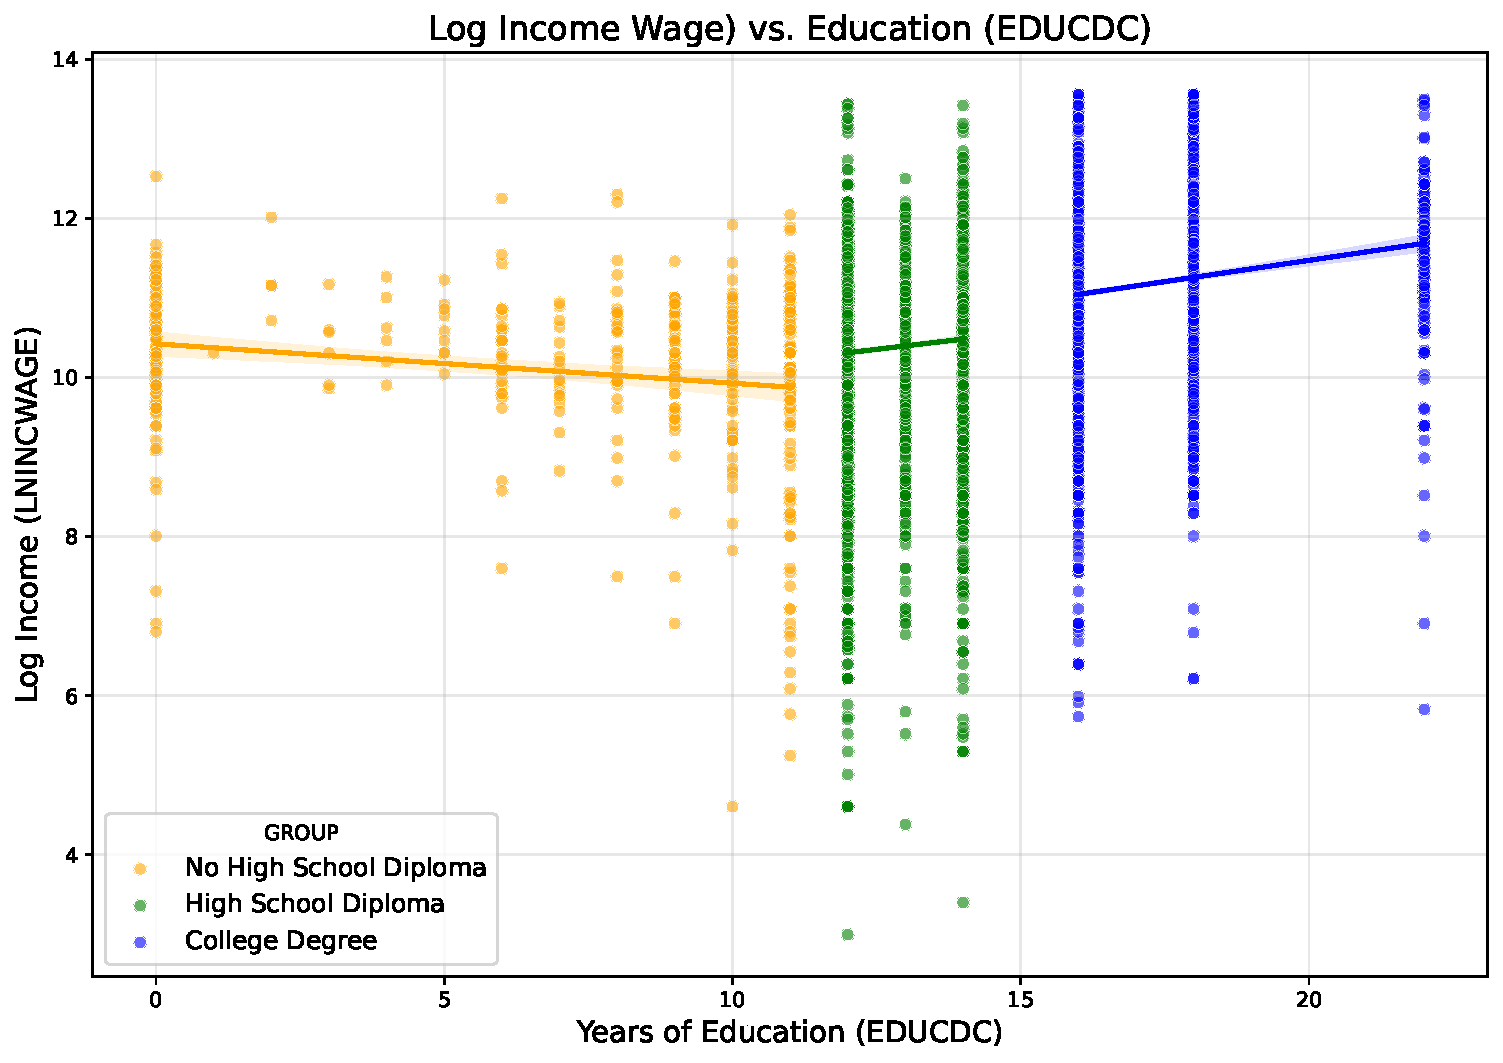
\includegraphics{mp1_files/figure-pdf/cell-26-output-1.pdf}

4.5a LNINCNWAGES = beta0 + beta1(hsdip) + beta2(coldip) + beta3(educdc ×
hsdip) + beta4(educdc × coldip) + beta5(age) + beta6(age\^{}2) +
beta7(female) + beta8(white) + beta9(black) + beta10(hispanic) +
beta11(married) + beta12(nchild) + beta13(vet) + epsilon

Using theory, intuition, and/or common sense, explain/justify why you
think your model is the best possible representation of the way the
world works (in other words, why you think you are correctly modeling f
(X) but not over-fitting e).

By now including the dummy variables for HSDIP, COLDIP and their
interaction terms with EDUCDC, the regression model can show
differential returns to education based on educational attainment. We
increase flexibbility of the model. Now, there can be different slopes
for the relationship between educational attainment and wage. It shows
us potential ``sheepskin effects'', so we can see the added value of
completing a HS or College--the degrees have a signalling effect that
help employers quickly screen competence.
https://www.econlib.org/archives/2012/01/the\_present\_val.html

4.5b

\begin{Shaded}
\begin{Highlighting}[]
\NormalTok{NEW\_reg }\OperatorTok{=}\NormalTok{ smf.ols(}
    \StringTok{\textquotesingle{}LNINCWAGE \textasciitilde{} HSDIP + COLDIP + HSDIP\_EDUCDC + COLDIP\_EDUCDC + FEMALE + AGE + AGEQ + WHITE + BLACK + HISPANIC+ MAR + NCHILD + VET\textquotesingle{}}\NormalTok{, data}\OperatorTok{=}\NormalTok{acs\_data).fit()}
\BuiltInTok{print}\NormalTok{(NEW\_reg.summary())}
\end{Highlighting}
\end{Shaded}

\begin{verbatim}
                            OLS Regression Results                            
==============================================================================
Dep. Variable:              LNINCWAGE   R-squared:                       0.306
Model:                            OLS   Adj. R-squared:                  0.305
Method:                 Least Squares   F-statistic:                     292.0
Date:                Thu, 30 Jan 2025   Prob (F-statistic):               0.00
Time:                        22:58:09   Log-Likelihood:                -11296.
No. Observations:                8610   AIC:                         2.262e+04
Df Residuals:                    8596   BIC:                         2.272e+04
Df Model:                          13                                         
Covariance Type:            nonrobust                                         
=================================================================================
                    coef    std err          t      P>|t|      [0.025      0.975]
---------------------------------------------------------------------------------
Intercept         7.1693      0.118     60.790      0.000       6.938       7.401
HSDIP            -0.7122      0.189     -3.761      0.000      -1.083      -0.341
COLDIP           -0.1929      0.177     -1.090      0.276      -0.540       0.154
HSDIP_EDUCDC      0.0833      0.014      5.855      0.000       0.055       0.111
COLDIP_EDUCDC     0.0708      0.010      7.063      0.000       0.051       0.090
FEMALE           -0.3967      0.020    -20.056      0.000      -0.435      -0.358
AGE               0.1368      0.006     24.069      0.000       0.126       0.148
AGEQ             -0.0014    6.7e-05    -21.149      0.000      -0.002      -0.001
WHITE             0.0238      0.027      0.875      0.382      -0.030       0.077
BLACK            -0.0745      0.042     -1.756      0.079      -0.158       0.009
HISPANIC         -0.0090      0.032     -0.278      0.781      -0.073       0.055
MAR               0.1833      0.023      8.039      0.000       0.139       0.228
NCHILD           -0.0029      0.010     -0.290      0.772      -0.023       0.017
VET               0.0199      0.050      0.399      0.690      -0.078       0.117
==============================================================================
Omnibus:                     2730.221   Durbin-Watson:                   1.856
Prob(Omnibus):                  0.000   Jarque-Bera (JB):            13032.061
Skew:                          -1.465   Prob(JB):                         0.00
Kurtosis:                       8.267   Cond. No.                     4.41e+04
==============================================================================

Notes:
[1] Standard Errors assume that the covariance matrix of the errors is correctly specified.
[2] The condition number is large, 4.41e+04. This might indicate that there are
strong multicollinearity or other numerical problems.
\end{verbatim}

REsults: The following variables are statistically significant at the
10\% level: HSDIP, HSDIP\_EDUCDC, COLDIP\_EDUCDC, FEMALE, AGE, AGEQ,
BLACK.

Importantly, our interaction terms proved to be statistically
significant, confirming the sheepskin effect or the idea that an HS
degree and a college degree bumps up wages.

4.5c

\begin{Shaded}
\begin{Highlighting}[]
\CommentTok{\# 22 year old, female, not white, black or hispanic. Not married, no children, not a veteran, HSDIP.}
\CommentTok{\# vs all else equal, but COLDIP}
\NormalTok{female\_1 }\OperatorTok{=}\NormalTok{ acs\_data.loc[}
\NormalTok{    (acs\_data[}\StringTok{\textquotesingle{}AGE\textquotesingle{}}\NormalTok{] }\OperatorTok{==} \DecValTok{22}\NormalTok{) }\OperatorTok{\&}\NormalTok{ (acs\_data[}\StringTok{\textquotesingle{}FEMALE\textquotesingle{}}\NormalTok{] }\OperatorTok{==} \DecValTok{1}\NormalTok{) }\OperatorTok{\&}\NormalTok{ (acs\_data[}\StringTok{\textquotesingle{}WHITE\textquotesingle{}}\NormalTok{] }\OperatorTok{==} \DecValTok{0}\NormalTok{) }\OperatorTok{\&}\NormalTok{ (}
\NormalTok{        acs\_data[}\StringTok{\textquotesingle{}BLACK\textquotesingle{}}\NormalTok{] }\OperatorTok{==} \DecValTok{0}\NormalTok{) }\OperatorTok{\&}\NormalTok{ (acs\_data[}\StringTok{\textquotesingle{}NCHILD\textquotesingle{}}\NormalTok{] }\OperatorTok{==} \DecValTok{0}\NormalTok{) }\OperatorTok{\&}\NormalTok{ (acs\_data[}\StringTok{\textquotesingle{}VET\textquotesingle{}}\NormalTok{] }\OperatorTok{==} \DecValTok{0}\NormalTok{) }\OperatorTok{\&}\NormalTok{ (acs\_data[}\StringTok{\textquotesingle{}MAR\textquotesingle{}}\NormalTok{] }\OperatorTok{==} \DecValTok{0}\NormalTok{) }\OperatorTok{\&}\NormalTok{ (acs\_data[}\StringTok{\textquotesingle{}HSDIP\textquotesingle{}}\NormalTok{] }\OperatorTok{==} \DecValTok{1}\NormalTok{) }\OperatorTok{\&}\NormalTok{ (acs\_data[}\StringTok{\textquotesingle{}COLDIP\textquotesingle{}}\NormalTok{] }\OperatorTok{==} \DecValTok{0}\NormalTok{) }\OperatorTok{\&}\NormalTok{ (acs\_data[}\StringTok{\textquotesingle{}HSDIP\_EDUCDC\textquotesingle{}}\NormalTok{] }\OperatorTok{==} \DecValTok{12}\NormalTok{)}\OperatorTok{\&}\NormalTok{ (acs\_data[}\StringTok{\textquotesingle{}COLDIP\_EDUCDC\textquotesingle{}}\NormalTok{] }\OperatorTok{==} \DecValTok{0}\NormalTok{)}
\NormalTok{]}
\CommentTok{\# Expectation }
\NormalTok{female\_1\_prediction }\OperatorTok{=}\NormalTok{ LNINCWAGE\_reg.get\_prediction(female\_1)}
\CommentTok{\# Display prediction summary}
\NormalTok{prediction\_summary }\OperatorTok{=}\NormalTok{ female\_1\_prediction.summary\_frame(alpha}\OperatorTok{=}\FloatTok{0.05}\NormalTok{)}
\BuiltInTok{print}\NormalTok{(prediction\_summary)}

\CommentTok{\# Convert log wages to actual wages}
\NormalTok{predicted\_wage }\OperatorTok{=}\NormalTok{ np.exp(prediction\_summary[}\StringTok{\textquotesingle{}mean\textquotesingle{}}\NormalTok{][}\DecValTok{0}\NormalTok{])}
\BuiltInTok{print}\NormalTok{(}\SpecialStringTok{f"Predicted wage with a high school diploma: $}\SpecialCharTok{\{}\NormalTok{predicted\_wage}\SpecialCharTok{:.2f\}}\SpecialStringTok{"}\NormalTok{)}

\CommentTok{\# alpha : significance level for the confidence interval.}
\CommentTok{\# Fix alpha to 0.05 so that the confidence interval should have 95\% coverage.}
\end{Highlighting}
\end{Shaded}

\begin{verbatim}
    mean  mean_se  mean_ci_lower  mean_ci_upper  obs_ci_lower  obs_ci_upper
0  9.470    0.035          9.402          9.539         7.675        11.265
1  9.470    0.035          9.402          9.539         7.675        11.265
2  9.449    0.033          9.385          9.513         7.655        11.244
3  9.449    0.033          9.385          9.513         7.655        11.244
4  9.470    0.035          9.402          9.539         7.675        11.265
5  9.449    0.033          9.385          9.513         7.655        11.244
6  9.449    0.033          9.385          9.513         7.655        11.244
7  9.449    0.033          9.385          9.513         7.655        11.244
8  9.470    0.035          9.402          9.539         7.675        11.265
9  9.449    0.033          9.385          9.513         7.655        11.244
10 9.449    0.033          9.385          9.513         7.655        11.244
11 9.449    0.033          9.385          9.513         7.655        11.244
12 9.470    0.035          9.402          9.539         7.675        11.265
Predicted wage with a high school diploma: $12966.88
\end{verbatim}

COLDIP

\begin{Shaded}
\begin{Highlighting}[]
\CommentTok{\# 22 year old, female, not white, black or hispanic. Not married, no children, not a veteran, HSDIP.}
\CommentTok{\# vs all else equal, but COLDIP}
\NormalTok{female\_2 }\OperatorTok{=}\NormalTok{ acs\_data.loc[}
\NormalTok{    (acs\_data[}\StringTok{\textquotesingle{}AGE\textquotesingle{}}\NormalTok{] }\OperatorTok{==} \DecValTok{22}\NormalTok{) }\OperatorTok{\&}\NormalTok{ (acs\_data[}\StringTok{\textquotesingle{}FEMALE\textquotesingle{}}\NormalTok{] }\OperatorTok{==} \DecValTok{1}\NormalTok{) }\OperatorTok{\&}\NormalTok{ (acs\_data[}\StringTok{\textquotesingle{}WHITE\textquotesingle{}}\NormalTok{] }\OperatorTok{==} \DecValTok{0}\NormalTok{) }\OperatorTok{\&}\NormalTok{ (}
\NormalTok{        acs\_data[}\StringTok{\textquotesingle{}BLACK\textquotesingle{}}\NormalTok{] }\OperatorTok{==} \DecValTok{0}\NormalTok{) }\OperatorTok{\&}\NormalTok{ (acs\_data[}\StringTok{\textquotesingle{}NCHILD\textquotesingle{}}\NormalTok{] }\OperatorTok{==} \DecValTok{0}\NormalTok{) }\OperatorTok{\&}\NormalTok{ (acs\_data[}\StringTok{\textquotesingle{}VET\textquotesingle{}}\NormalTok{] }\OperatorTok{==} \DecValTok{0}\NormalTok{) }\OperatorTok{\&}\NormalTok{ (acs\_data[}\StringTok{\textquotesingle{}MAR\textquotesingle{}}\NormalTok{] }\OperatorTok{==} \DecValTok{0}\NormalTok{) }\OperatorTok{\&}\NormalTok{ (acs\_data[}\StringTok{\textquotesingle{}HSDIP\textquotesingle{}}\NormalTok{] }\OperatorTok{==} \DecValTok{0}\NormalTok{) }\OperatorTok{\&}\NormalTok{ (acs\_data[}\StringTok{\textquotesingle{}COLDIP\textquotesingle{}}\NormalTok{] }\OperatorTok{==} \DecValTok{1}\NormalTok{) }\OperatorTok{\&}\NormalTok{ (acs\_data[}\StringTok{\textquotesingle{}HSDIP\_EDUCDC\textquotesingle{}}\NormalTok{] }\OperatorTok{==} \DecValTok{0}\NormalTok{)}\OperatorTok{\&}\NormalTok{ (acs\_data[}\StringTok{\textquotesingle{}COLDIP\_EDUCDC\textquotesingle{}}\NormalTok{] }\OperatorTok{==} \DecValTok{16}\NormalTok{)}
\NormalTok{]}
\CommentTok{\# Expectation }
\NormalTok{female\_2\_prediction }\OperatorTok{=}\NormalTok{ LNINCWAGE\_reg.get\_prediction(female\_2)}
\CommentTok{\# Display prediction summary}
\NormalTok{prediction\_summary\_2 }\OperatorTok{=}\NormalTok{ female\_2\_prediction.summary\_frame(alpha}\OperatorTok{=}\FloatTok{0.05}\NormalTok{)}
\BuiltInTok{print}\NormalTok{(prediction\_summary\_2)}

\CommentTok{\# Convert log wages to actual wages}
\NormalTok{predicted\_wage\_2 }\OperatorTok{=}\NormalTok{ np.exp(prediction\_summary\_2[}\StringTok{\textquotesingle{}mean\textquotesingle{}}\NormalTok{][}\DecValTok{0}\NormalTok{])}
\BuiltInTok{print}\NormalTok{(}\SpecialStringTok{f"Predicted wage with a college diploma: $}\SpecialCharTok{\{}\NormalTok{predicted\_wage\_2}\SpecialCharTok{:.2f\}}\SpecialStringTok{"}\NormalTok{)}

\CommentTok{\# alpha : significance level for the confidence interval.}
\CommentTok{\# Fix alpha to 0.05 so that the confidence interval should have 95\% coverage.}
\end{Highlighting}
\end{Shaded}

\begin{verbatim}
   mean  mean_se  mean_ci_lower  mean_ci_upper  obs_ci_lower  obs_ci_upper
0 9.868    0.035          9.800          9.936         8.073        11.662
1 9.868    0.035          9.800          9.936         8.073        11.662
2 9.847    0.035          9.779          9.915         8.052        11.641
3 9.868    0.035          9.800          9.936         8.073        11.662
4 9.847    0.035          9.779          9.915         8.052        11.641
5 9.847    0.035          9.779          9.915         8.052        11.641
6 9.868    0.035          9.800          9.936         8.073        11.662
7 9.868    0.035          9.800          9.936         8.073        11.662
8 9.868    0.035          9.800          9.936         8.073        11.662
9 9.868    0.035          9.800          9.936         8.073        11.662
Predicted wage with a college diploma: $19299.12
\end{verbatim}

4.5d Those with college degrees have a higher predicted wage than those
without. They earn about 6, 332 USD more on average.

4.5e SInce we know that a college degree will increase the average
expected wage , it would be good to create policy to expand access to
college education. Howeever, what our model does is to test correlation
and not causation, so we do need to consider how other factors influence
this (ommitted variables like household size or grades in school). The
legislation should also try to ensure access to good quality education
and ensure that The quality and type of education matter, not just
access. ANd we should consider who (race, gender, origin, socioeconomic
status) is being provided with this subsidy.

4.5f

\begin{Shaded}
\begin{Highlighting}[]
\NormalTok{NEW\_reg\_r\_squared }\OperatorTok{=}\NormalTok{ NEW\_reg.rsquared}
\NormalTok{NEW\_reg\_adjusted\_r\_squared }\OperatorTok{=} \BuiltInTok{round}\NormalTok{(NEW\_reg.rsquared\_adj,}\DecValTok{4}\NormalTok{)}

\BuiltInTok{print}\NormalTok{(}\SpecialStringTok{f"R{-}squared: }\SpecialCharTok{\{}\NormalTok{NEW\_reg\_r\_squared}\SpecialCharTok{:.4f\}}\SpecialStringTok{"}\NormalTok{)}
\BuiltInTok{print}\NormalTok{(}\SpecialStringTok{f"}\SpecialCharTok{\{}\NormalTok{(NEW\_reg\_adjusted\_r\_squared}\OperatorTok{*}\DecValTok{100}\NormalTok{)}\SpecialCharTok{\}}\SpecialStringTok{ percent of the variation in logwages can be explained by the model"}\NormalTok{)}
\end{Highlighting}
\end{Shaded}

\begin{verbatim}
R-squared: 0.3063
30.53 percent of the variation in logwages can be explained by the model
\end{verbatim}

versus

\begin{Shaded}
\begin{Highlighting}[]
\NormalTok{OLD\_reg\_r\_squared }\OperatorTok{=}\NormalTok{ LNINCWAGE\_reg.rsquared}
\NormalTok{OLD\_reg\_adjusted\_r\_squared }\OperatorTok{=}\NormalTok{ LNINCWAGE\_reg.rsquared\_adj}

\BuiltInTok{print}\NormalTok{(}\SpecialStringTok{f"R{-}squared: }\SpecialCharTok{\{}\NormalTok{OLD\_reg\_r\_squared}\SpecialCharTok{:.4f\}}\SpecialStringTok{"}\NormalTok{)}
\BuiltInTok{print}\NormalTok{(}\SpecialStringTok{f"Adjusted R{-}squared: }\SpecialCharTok{\{}\NormalTok{OLD\_reg\_adjusted\_r\_squared}\SpecialCharTok{:.4f\}}\SpecialStringTok{"}\NormalTok{)}
\end{Highlighting}
\end{Shaded}

\begin{verbatim}
R-squared: 0.2817
Adjusted R-squared: 0.2809
\end{verbatim}

We see that the new model has a higher R 2 and adjusted R2, meaning it
better explains the variation in log wages compared to the model from 3.

4.5g

For both 22 year olds, the CIs are pretty narrow, meaning the estimates
are likely quite precise. High school diploma, the model predicts a log
wage of 9.470154 with a 95\% confidence interval of {[}9.401522,
9.538785{]}. For the college graduate, the predicted log wage is
9.867815 with a confidence interval of {[}9.799870, 9.935759{]}. But,
the model only explains 30.53\% of the variation in log wages, so
there's still quite a bit of variation that is not explained.

So, while our model is quite precise, we must be wary. We may need to
explore a bit more and use data from previous years as well.

4.6a

\begin{Shaded}
\begin{Highlighting}[]
\CommentTok{\# Predictors from Question 3 (excluding AGE and AGE\_SQUARED)}
\NormalTok{predictors\_q3 }\OperatorTok{=}\NormalTok{ [}\StringTok{"EDUCDC"}\NormalTok{, }\StringTok{"FEMALE"}\NormalTok{, }\StringTok{"WHITE"}\NormalTok{, }\StringTok{"BLACK"}\NormalTok{, }\StringTok{"HISPANIC"}\NormalTok{, }
                 \StringTok{"MAR"}\NormalTok{, }\StringTok{"NCHILD"}\NormalTok{, }\StringTok{"VET"}\NormalTok{]}

\CommentTok{\# Define the age variable and the target variable}
\NormalTok{X\_age }\OperatorTok{=}\NormalTok{ acs\_data[[}\StringTok{"AGE"}\NormalTok{]]}
\NormalTok{y }\OperatorTok{=}\NormalTok{ acs\_data[}\StringTok{"LNINCWAGE"}\NormalTok{]}

\CommentTok{\# Define the knots for the spline (18 and 65)}
\NormalTok{knots }\OperatorTok{=}\NormalTok{ np.array([}\DecValTok{18}\NormalTok{, }\DecValTok{65}\NormalTok{]).reshape(}\OperatorTok{{-}}\DecValTok{1}\NormalTok{, }\DecValTok{1}\NormalTok{)}

\CommentTok{\# Create the spline transformer}
\NormalTok{spline\_transformer }\OperatorTok{=}\NormalTok{ SplineTransformer(degree}\OperatorTok{=}\DecValTok{3}\NormalTok{, knots}\OperatorTok{=}\NormalTok{knots, include\_bias}\OperatorTok{=}\VariableTok{False}\NormalTok{)}

\CommentTok{\# Transform the age variable using the spline}
\NormalTok{X\_splines }\OperatorTok{=}\NormalTok{ spline\_transformer.fit\_transform(X\_age)}

\CommentTok{\# Combine the spline{-}transformed age variable with the other predictors}
\NormalTok{X\_controls }\OperatorTok{=}\NormalTok{ acs\_data[predictors\_q3]}
\NormalTok{X }\OperatorTok{=}\NormalTok{ np.hstack([X\_splines, X\_controls])}

\CommentTok{\# Fit the linear regression model}
\NormalTok{model }\OperatorTok{=}\NormalTok{ LinearRegression()}
\NormalTok{model.fit(X, y)}

\CommentTok{\# Print the intercept and coefficients}
\BuiltInTok{print}\NormalTok{(}\StringTok{"Intercept:"}\NormalTok{, model.intercept\_)}
\NormalTok{spline\_columns }\OperatorTok{=}\NormalTok{ [}\SpecialStringTok{f"spline\_}\SpecialCharTok{\{}\NormalTok{i}\SpecialCharTok{\}}\SpecialStringTok{"} \ControlFlowTok{for}\NormalTok{ i }\KeywordTok{in} \BuiltInTok{range}\NormalTok{(X\_splines.shape[}\DecValTok{1}\NormalTok{])]}
\NormalTok{all\_columns }\OperatorTok{=}\NormalTok{ spline\_columns }\OperatorTok{+}\NormalTok{ predictors\_q3}
\NormalTok{coefficients }\OperatorTok{=}\NormalTok{ pd.Series(model.coef\_, index}\OperatorTok{=}\NormalTok{all\_columns)}
\BuiltInTok{print}\NormalTok{(}\StringTok{"Coefficients:"}\NormalTok{)}
\BuiltInTok{print}\NormalTok{(coefficients)}

\CommentTok{\# Calculate the adjusted R{-}squared}
\NormalTok{r\_squared }\OperatorTok{=}\NormalTok{ model.score(X, y)}
\NormalTok{n }\OperatorTok{=} \BuiltInTok{len}\NormalTok{(y)}
\NormalTok{p }\OperatorTok{=}\NormalTok{ X.shape[}\DecValTok{1}\NormalTok{]}
\NormalTok{adjusted\_r\_squared }\OperatorTok{=} \DecValTok{1} \OperatorTok{{-}}\NormalTok{ ((}\DecValTok{1} \OperatorTok{{-}}\NormalTok{ r\_squared) }\OperatorTok{*}\NormalTok{ (n }\OperatorTok{{-}} \DecValTok{1}\NormalTok{)) }\OperatorTok{/}\NormalTok{ (n }\OperatorTok{{-}}\NormalTok{ p }\OperatorTok{{-}} \DecValTok{1}\NormalTok{)}
\BuiltInTok{print}\NormalTok{(}\StringTok{"The Adjusted R{-}squared of the model with the two age knots is"}\NormalTok{, adjusted\_r\_squared)}
\end{Highlighting}
\end{Shaded}

\begin{verbatim}
Intercept: 14.075815645865092
Coefficients:
spline_0   -22.189
spline_1    -1.931
spline_2    -6.236
EDUCDC       0.096
FEMALE      -0.379
WHITE       -0.013
BLACK       -0.130
HISPANIC    -0.028
MAR          0.190
NCHILD      -0.008
VET         -0.016
dtype: float64
The Adjusted R-squared of the model with the two age knots is 0.2914488777671098
\end{verbatim}

4.6b The adjusted R2 of .291 is slightly higher than the one inmodel 3.
The adjusted R2 of .291 is higher than the one inmodel 3. This is
probably because, as we learned, splines capture nonlinear
relationsships. In this case, the nonlinear effects of age, which thus
improves the model's fit (it explains more of the vairaion).

4.6c

\begin{Shaded}
\begin{Highlighting}[]
\CommentTok{\# Define the knots for the spline (24 and 55)}
\NormalTok{knots\_24\_55 }\OperatorTok{=}\NormalTok{ np.array([}\DecValTok{24}\NormalTok{, }\DecValTok{55}\NormalTok{]).reshape(}\OperatorTok{{-}}\DecValTok{1}\NormalTok{, }\DecValTok{1}\NormalTok{)}

\CommentTok{\# Create the spline transformer}
\NormalTok{spline\_transformer\_24\_55 }\OperatorTok{=}\NormalTok{ SplineTransformer(degree}\OperatorTok{=}\DecValTok{3}\NormalTok{, knots}\OperatorTok{=}\NormalTok{knots\_24\_55, include\_bias}\OperatorTok{=}\VariableTok{False}\NormalTok{)}

\CommentTok{\# Transform the age variable using the spline}
\NormalTok{X\_splines\_24\_55 }\OperatorTok{=}\NormalTok{ spline\_transformer\_24\_55.fit\_transform(X\_age)}

\CommentTok{\# Combine the spline{-}transformed age variable with the other predictors}
\NormalTok{X\_24\_55 }\OperatorTok{=}\NormalTok{ np.hstack([X\_splines\_24\_55, X\_controls])}

\CommentTok{\# Fit the linear regression model}
\NormalTok{model\_24\_55 }\OperatorTok{=}\NormalTok{ LinearRegression()}
\NormalTok{model\_24\_55.fit(X\_24\_55, y)}

\CommentTok{\# Print the intercept and coefficients}
\BuiltInTok{print}\NormalTok{(}\StringTok{"Intercept (knots at 24 and 55):"}\NormalTok{, model\_24\_55.intercept\_)}
\NormalTok{spline\_columns\_24\_55 }\OperatorTok{=}\NormalTok{ [}\SpecialStringTok{f"spline\_24\_55\_}\SpecialCharTok{\{}\NormalTok{i}\SpecialCharTok{\}}\SpecialStringTok{"} \ControlFlowTok{for}\NormalTok{ i }\KeywordTok{in} \BuiltInTok{range}\NormalTok{(X\_splines\_24\_55.shape[}\DecValTok{1}\NormalTok{])]}
\NormalTok{all\_columns\_24\_55 }\OperatorTok{=}\NormalTok{ spline\_columns\_24\_55 }\OperatorTok{+}\NormalTok{ predictors\_q3}
\NormalTok{coefficients\_24\_55 }\OperatorTok{=}\NormalTok{ pd.Series(model\_24\_55.coef\_, index}\OperatorTok{=}\NormalTok{all\_columns\_24\_55)}
\BuiltInTok{print}\NormalTok{(}\StringTok{"Coefficients (knots at 24 and 55):"}\NormalTok{)}
\BuiltInTok{print}\NormalTok{(coefficients\_24\_55)}

\CommentTok{\# Calculate the adjusted R{-}squared}
\NormalTok{r\_squared\_24\_55 }\OperatorTok{=}\NormalTok{ model\_24\_55.score(X\_24\_55, y)}
\NormalTok{n\_24\_55 }\OperatorTok{=} \BuiltInTok{len}\NormalTok{(y)}
\NormalTok{p\_24\_55 }\OperatorTok{=}\NormalTok{ X\_24\_55.shape[}\DecValTok{1}\NormalTok{]}
\NormalTok{adjusted\_r\_squared\_24\_55 }\OperatorTok{=} \DecValTok{1} \OperatorTok{{-}}\NormalTok{ ((}\DecValTok{1} \OperatorTok{{-}}\NormalTok{ r\_squared\_24\_55) }\OperatorTok{*}\NormalTok{ (n\_24\_55 }\OperatorTok{{-}} \DecValTok{1}\NormalTok{)) }\OperatorTok{/}\NormalTok{ (n\_24\_55 }\OperatorTok{{-}}\NormalTok{ p\_24\_55 }\OperatorTok{{-}} \DecValTok{1}\NormalTok{)}
\BuiltInTok{print}\NormalTok{(}\StringTok{"Adjusted R{-}squared (knots at 24 and 55):"}\NormalTok{, adjusted\_r\_squared\_24\_55)}
\end{Highlighting}
\end{Shaded}

\begin{verbatim}
Intercept (knots at 24 and 55): 12.615808625187793
Coefficients (knots at 24 and 55):
spline_24_55_0   -13.896
spline_24_55_1    -1.510
spline_24_55_2    -4.272
EDUCDC             0.102
FEMALE            -0.385
WHITE             -0.015
BLACK             -0.127
HISPANIC          -0.016
MAR                0.211
NCHILD             0.008
VET               -0.019
dtype: float64
Adjusted R-squared (knots at 24 and 55): 0.2673685975131527
\end{verbatim}

Model of my choosing

\begin{Shaded}
\begin{Highlighting}[]
\CommentTok{\# Knots for the spline (21 and 65)}
\NormalTok{knots\_21\_65 }\OperatorTok{=}\NormalTok{ np.array([}\DecValTok{21}\NormalTok{, }\DecValTok{65}\NormalTok{]).reshape(}\OperatorTok{{-}}\DecValTok{1}\NormalTok{, }\DecValTok{1}\NormalTok{)}

\CommentTok{\# Create the spline transformer}
\NormalTok{spline\_transformer\_21\_65 }\OperatorTok{=}\NormalTok{ SplineTransformer(degree}\OperatorTok{=}\DecValTok{3}\NormalTok{, knots}\OperatorTok{=}\NormalTok{knots\_21\_65, include\_bias}\OperatorTok{=}\VariableTok{False}\NormalTok{)}

\CommentTok{\# Transform the age variable using the spline}
\NormalTok{X\_splines\_21\_65 }\OperatorTok{=}\NormalTok{ spline\_transformer\_21\_65.fit\_transform(X\_age)}

\CommentTok{\# Combine the spline{-}transformed age variable with the other predictors}
\NormalTok{X\_21\_65 }\OperatorTok{=}\NormalTok{ np.hstack([X\_splines\_21\_65, X\_controls])}

\CommentTok{\# Fit the linear regression model}
\NormalTok{model\_21\_65 }\OperatorTok{=}\NormalTok{ LinearRegression()}
\NormalTok{model\_21\_65.fit(X\_21\_65, y)}

\CommentTok{\# Print the intercept and coefficients}
\BuiltInTok{print}\NormalTok{(}\StringTok{"Intercept (knots at 21 and 65):"}\NormalTok{, model\_21\_65.intercept\_)}
\NormalTok{spline\_columns\_21\_65 }\OperatorTok{=}\NormalTok{ [}\SpecialStringTok{f"spline\_21\_65\_}\SpecialCharTok{\{}\NormalTok{i}\SpecialCharTok{\}}\SpecialStringTok{"} \ControlFlowTok{for}\NormalTok{ i }\KeywordTok{in} \BuiltInTok{range}\NormalTok{(X\_splines\_21\_65.shape[}\DecValTok{1}\NormalTok{])]}
\NormalTok{all\_columns\_21\_65 }\OperatorTok{=}\NormalTok{ spline\_columns\_21\_65 }\OperatorTok{+}\NormalTok{ predictors\_q3}
\NormalTok{coefficients\_21\_65 }\OperatorTok{=}\NormalTok{ pd.Series(model\_21\_65.coef\_, index}\OperatorTok{=}\NormalTok{all\_columns\_21\_65)}
\BuiltInTok{print}\NormalTok{(}\StringTok{"Coefficients (knots at 21 and 65):"}\NormalTok{)}
\BuiltInTok{print}\NormalTok{(coefficients\_21\_65)}

\CommentTok{\# Getting the ajusted R{-}squared}
\NormalTok{r\_squared\_21\_65 }\OperatorTok{=}\NormalTok{ model\_21\_65.score(X\_21\_65, y)}
\NormalTok{n\_21\_65 }\OperatorTok{=} \BuiltInTok{len}\NormalTok{(y)}
\NormalTok{p\_21\_65 }\OperatorTok{=}\NormalTok{ X\_21\_65.shape[}\DecValTok{1}\NormalTok{]}
\NormalTok{adjusted\_r\_squared\_21\_65 }\OperatorTok{=} \DecValTok{1} \OperatorTok{{-}}\NormalTok{ ((}\DecValTok{1} \OperatorTok{{-}}\NormalTok{ r\_squared\_21\_65) }\OperatorTok{*}\NormalTok{ (n\_21\_65 }\OperatorTok{{-}} \DecValTok{1}\NormalTok{)) }\OperatorTok{/}\NormalTok{ (n\_21\_65 }\OperatorTok{{-}}\NormalTok{ p\_21\_65 }\OperatorTok{{-}} \DecValTok{1}\NormalTok{)}
\BuiltInTok{print}\NormalTok{(}\StringTok{"Adjusted R{-}squared (knots at 21 and 65):"}\NormalTok{, adjusted\_r\_squared\_21\_65)}
\end{Highlighting}
\end{Shaded}

\begin{verbatim}
Intercept (knots at 21 and 65): 13.613217907092636
Coefficients (knots at 21 and 65):
spline_21_65_0   -18.378
spline_21_65_1    -1.803
spline_21_65_2    -5.629
EDUCDC             0.098
FEMALE            -0.380
WHITE             -0.013
BLACK             -0.127
HISPANIC          -0.022
MAR                0.198
NCHILD            -0.006
VET               -0.014
dtype: float64
Adjusted R-squared (knots at 21 and 65): 0.2819850168684307
\end{verbatim}

Since my model of 21 and 65 have a higher adjusted R2, it is a more
powerful model that fits the data better than the suggested one. I chose
21, thinking this is the age in which many students graduate from
university and 65 is when they retire, which would likely improve the
model.

4.6d

\begin{Shaded}
\begin{Highlighting}[]
\CommentTok{\# Create a test dataframe for predictions}
\NormalTok{df\_test }\OperatorTok{=}\NormalTok{ pd.DataFrame(\{}
    \StringTok{"EDUCDC"}\NormalTok{: [}\DecValTok{16}\NormalTok{, }\DecValTok{16}\NormalTok{],  }
    \StringTok{"FEMALE"}\NormalTok{: [}\DecValTok{1}\NormalTok{, }\DecValTok{1}\NormalTok{],     }
    \StringTok{"AGE"}\NormalTok{: [}\DecValTok{17}\NormalTok{, }\DecValTok{50}\NormalTok{],      }
    \StringTok{"WHITE"}\NormalTok{: [}\DecValTok{0}\NormalTok{, }\DecValTok{0}\NormalTok{],      }
    \StringTok{"BLACK"}\NormalTok{: [}\DecValTok{0}\NormalTok{, }\DecValTok{0}\NormalTok{],      }
    \StringTok{"HISPANIC"}\NormalTok{: [}\DecValTok{0}\NormalTok{, }\DecValTok{0}\NormalTok{],   }
    \StringTok{"MAR"}\NormalTok{: [}\DecValTok{0}\NormalTok{, }\DecValTok{0}\NormalTok{],   }
    \StringTok{"NCHILD"}\NormalTok{: [}\DecValTok{0}\NormalTok{, }\DecValTok{0}\NormalTok{],     }
    \StringTok{"VET"}\NormalTok{: [}\DecValTok{0}\NormalTok{, }\DecValTok{0}\NormalTok{]       }
\NormalTok{\})}

\CommentTok{\# Transform AGE into splines using the transformer from 6.c (knots at 24 and 55)}
\NormalTok{splines\_test }\OperatorTok{=}\NormalTok{ spline\_transformer\_24\_55.transform(df\_test[[}\StringTok{"AGE"}\NormalTok{]])}

\CommentTok{\# Combine spline{-}transformed AGE with other predictors from Question 3}
\NormalTok{X\_test }\OperatorTok{=}\NormalTok{ np.hstack([splines\_test, df\_test[predictors\_q3]])}

\CommentTok{\# Predict log wages using the model with knots at 24 and 55}
\NormalTok{log\_wage\_pred }\OperatorTok{=}\NormalTok{ model\_24\_55.predict(X\_test)}

\CommentTok{\# Convert log wages to actual wages}
\NormalTok{wage\_pred }\OperatorTok{=}\NormalTok{ np.exp(log\_wage\_pred)}

\CommentTok{\# Create a results dataframe}
\NormalTok{df\_pred }\OperatorTok{=}\NormalTok{ pd.DataFrame(\{}
    \StringTok{"AGE"}\NormalTok{: [}\DecValTok{17}\NormalTok{, }\DecValTok{50}\NormalTok{],}
    \StringTok{"Predicted Log Wage"}\NormalTok{: log\_wage\_pred,}
    \StringTok{"Predicted Wage"}\NormalTok{: wage\_pred}
\NormalTok{\})}

\BuiltInTok{print}\NormalTok{(df\_pred)}
\end{Highlighting}
\end{Shaded}

\begin{verbatim}
   AGE  Predicted Log Wage  Predicted Wage
0   17               9.824       18470.276
1   50              10.713       44950.928
\end{verbatim}

The knots in the spline let us reflect wage differences because of the
non-linear effects of age.

Here, we are assuming both the 17 and 50 year olds have 16 years of
education, even if it isn't really realistic. Predictably, the 17 year
olds, who have less work experience have lower predicted wage by around
31K USD. Meanwhile,at 50, one is likely at the top--a managing partner,
director, VP, department head, etc, making earnings much higher.




\end{document}
